\documentclass[12pt, a4paper]{article}


% A pretty common set of packages
\usepackage[margin=2.5cm]{geometry}
\usepackage[T1]{fontenc}
\usepackage{graphicx}
\usepackage{amssymb}
\usepackage{amsmath}
\usepackage{bm}
\usepackage{color}
\usepackage{float}
\usepackage{bm}
\usepackage{physics}
\usepackage{subcaption}

\DeclareRobustCommand{\uvec}[1]{{%
  \ifcsname uvec#1\endcsname
     \csname uvec#1\endcsname
   \else
    \bm{\hat{\mathbf{#1}}}%
   \fi
}}
\newcommand{\olsi}[1]{\,\overline{\!{#1}}} % overline short italic

\usepackage[colorlinks=true, 
    linkcolor=blue,          % color of internal links
    citecolor=blue,        % color of links to bibliography
    filecolor=blue,      % color of file links
    urlcolor=blue]{hyperref}

\title{[16-833] Homework 1 : Written Report}
\author{Bharath Somayajula, Christopher Klammer}
\date{\today}

\begin{document}

\maketitle

\tableofcontents

\clearpage

\section{Introduction}
For this homework, we implemented particle filter for localization of robot when the map is known. We used Python language for implementation. In the sections below we describe the details of motion model, sensor model, ray casting, resampling, parameter tuning and suggestions for future work.

\section{Motion Model}
\subsection{Description}
The motion model acts as the prediction step in the particle filter. We follow the odometry motion model mentioned in \cite{ProbRob} as shown below:


\begin{figure}[H]
  \center
  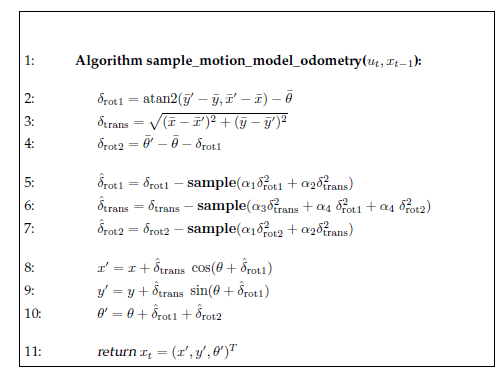
\includegraphics{OdometryMotionModel.png}
  \caption{Psuedocode for Odometry Motion Model \cite{ProbRob}}
\end{figure}

\noindent This algorithm assumes that two odometry measurements are given along with the previous state. The algorithm estimates the change in rotation and translation for the robot between time steps. This model also samples noise from a guassian distribution in order to add some perturbation. This perturbation allows uncertainity to be modelled and, in practice, allows particles to explore different paths. This approach, however, does require for the noise parameters to be tuned effectively in order to receive accurate localization.

\subsection{Implementation}
\begin{figure}[H]
  \begin{center}
    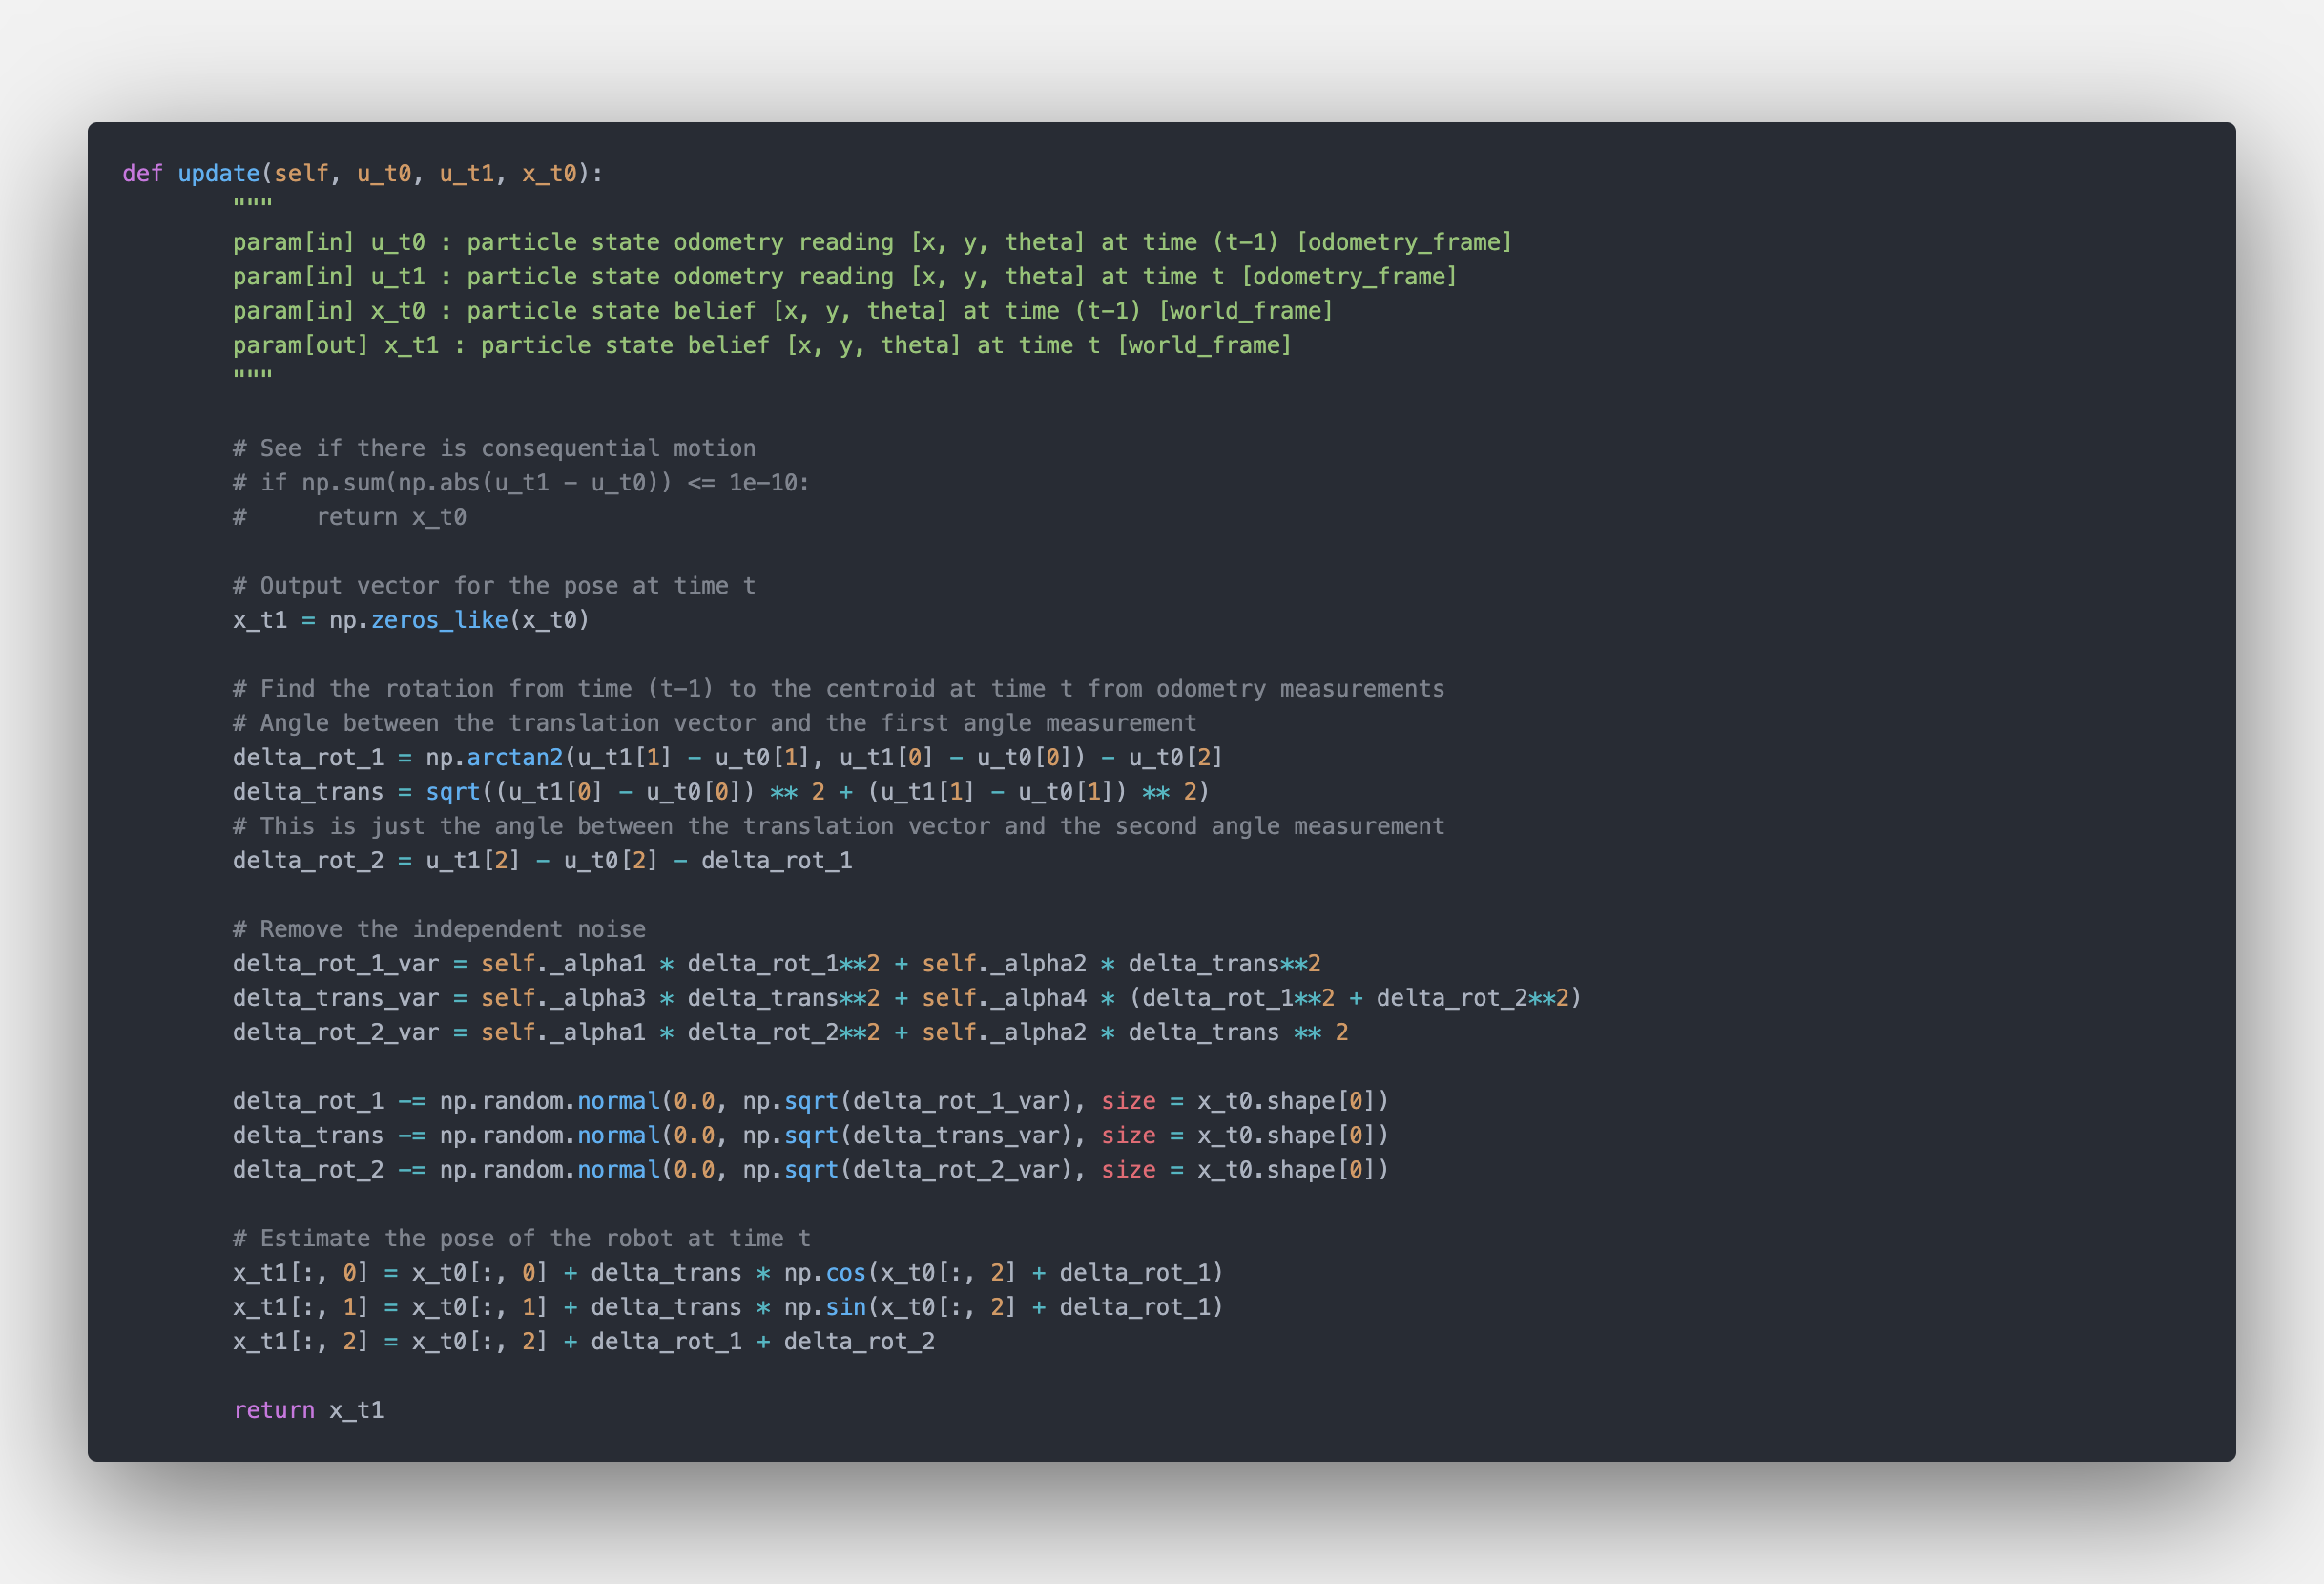
\includegraphics[width=1.0\textwidth]{./results/motion_model_2.png}
    \caption{Implementation of the Odometry Motion Model}
  \end{center}
\end{figure}

\subsection{Alterations}
One improvement made on this algorithm was adding a check on whether there was consequential motion before predicting the state.

\[ 
x_{t1} = \left\{
\begin{array}{ll}
    motion\_model\_odometry(u_{t-1}, u_t, x_{t-1}) & \lVert u_{t1} - u_{t0} \rVert > \tau \\
    x_{t0} & else
\end{array} 
\right. 
\]

\noindent That is, if there is consequential motion, we will run the prediciton step with the odometry motion model. Otherwise, we will not update the state estimate for the particle. We found this change to reduce the particle jitter and enforce a much more cohesive and smooth trajectory.

\clearpage
\section{Sensor Model}
\subsection{Ray Casting}
\subsubsection{Description}
RayCasting is needed for estimation of true ranges at various angles.\\\\ 
To make implementation easier, we created a \textit{RayCasting} module that performs ray casting. The \textit{get\_true\_ranges\_vec} function is invoked to compute ranges at various angles for all particles. \textit{sensor\_location} function adjusts the state of robots by $25$ cm to take into account the distance between robot and the sensor.
\subsubsection{Implementation}
Ray Casting is the most computationally expensive part of the code. We implemented the following changes to naive implementation of ray casting to improve the performance.

\begin{enumerate}
  \item To avoid redundant computations, we perform ray casting only once in constructor function using the \textit{relative\_ray\_casting} function. This function casts rays relative to the robot in it's canonical orientation. At all future time steps, the points along these rays are simply rotated and translated to match the position and orientation of robot! This led to massive gains in performance. The implementation of \textit{relative\_ray\_casting} function is shown below.
  \begin{itemize}
    \item 
    \begin{minipage}[t]{\linewidth}
      \vspace{0pt}
      \begin{center}
        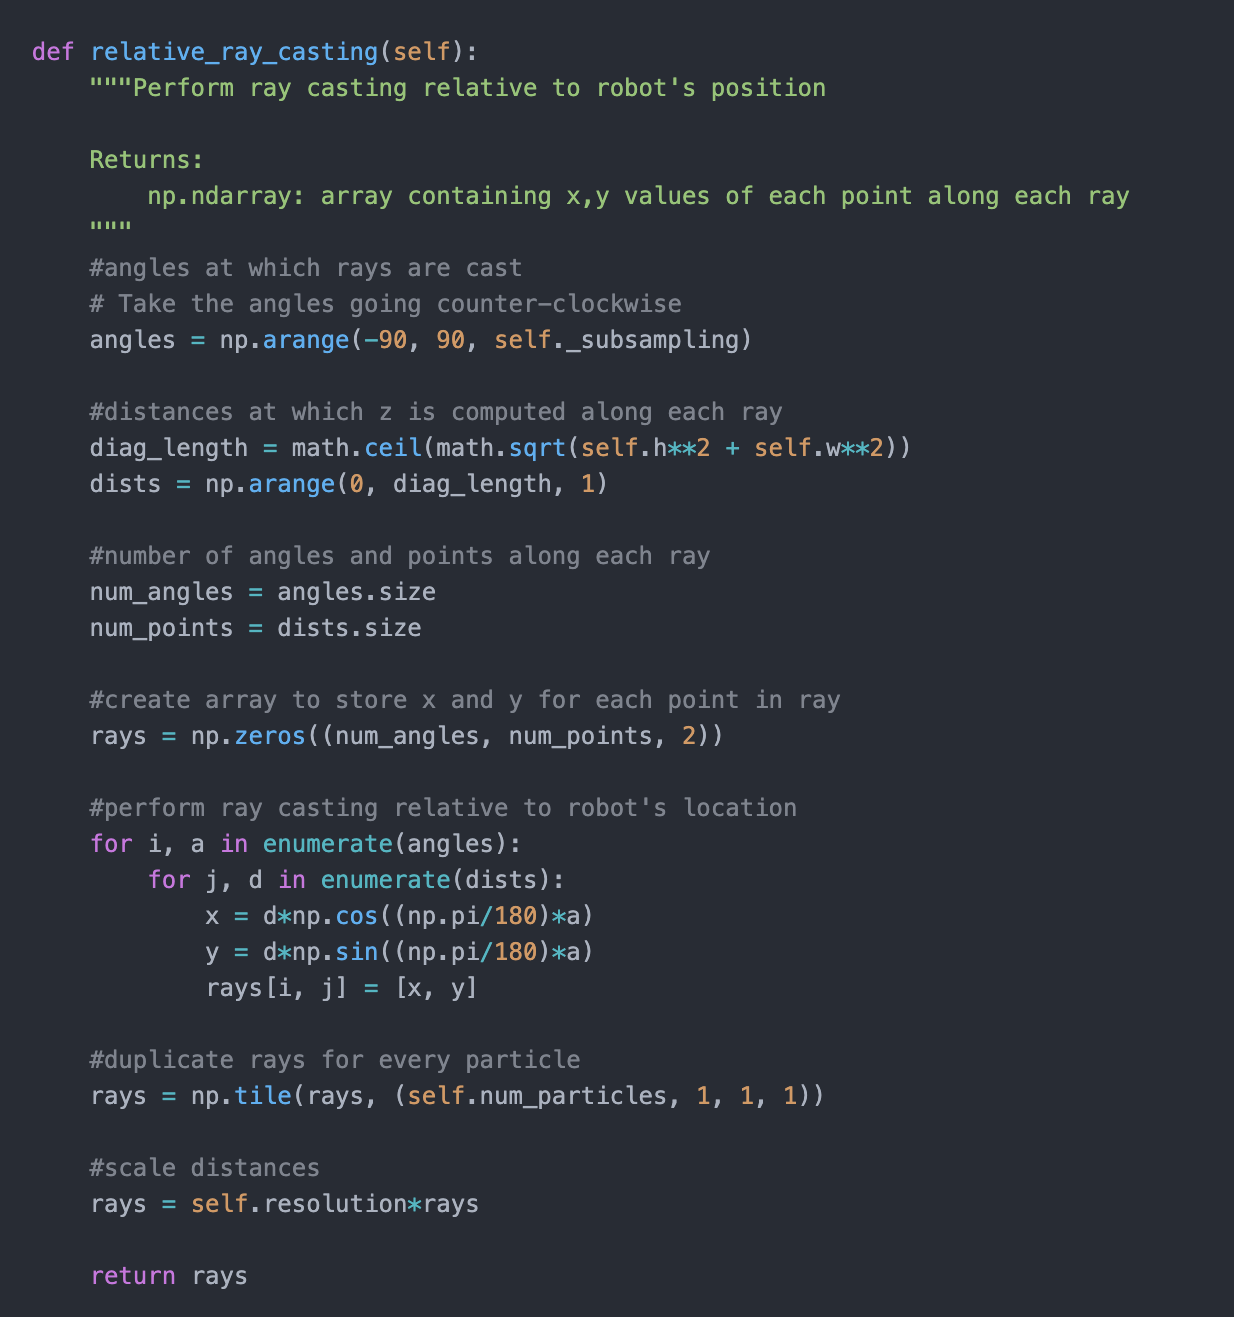
\includegraphics[scale=0.25]{./results/ray_casting_opt_1.png}
        \captionof{figure}{Pre-computation of points along rays}
        \label{fig:sm_1}
      \end{center}
    \end{minipage}
  \end{itemize}
  \item Once the rays have been oriented based on location and orientation of a particle, the logic used to measure the range along each ray at which it encounters an obstacle or goes out of the map has been vectorized. Compared to the naive implementation of this logic using nested for-loops, the fully vectorized implementation is approximately \textbf{9.5x faster}.  The vectorized logic is shown below
  \item Vectorize the code to enable computation of ranges for all particles simultaneously instead of performing ray casting in a loop seperately for each particle
  \begin{itemize}
    \item 
    \begin{minipage}[t]{\linewidth}
      \vspace{0pt}
      \begin{center}
        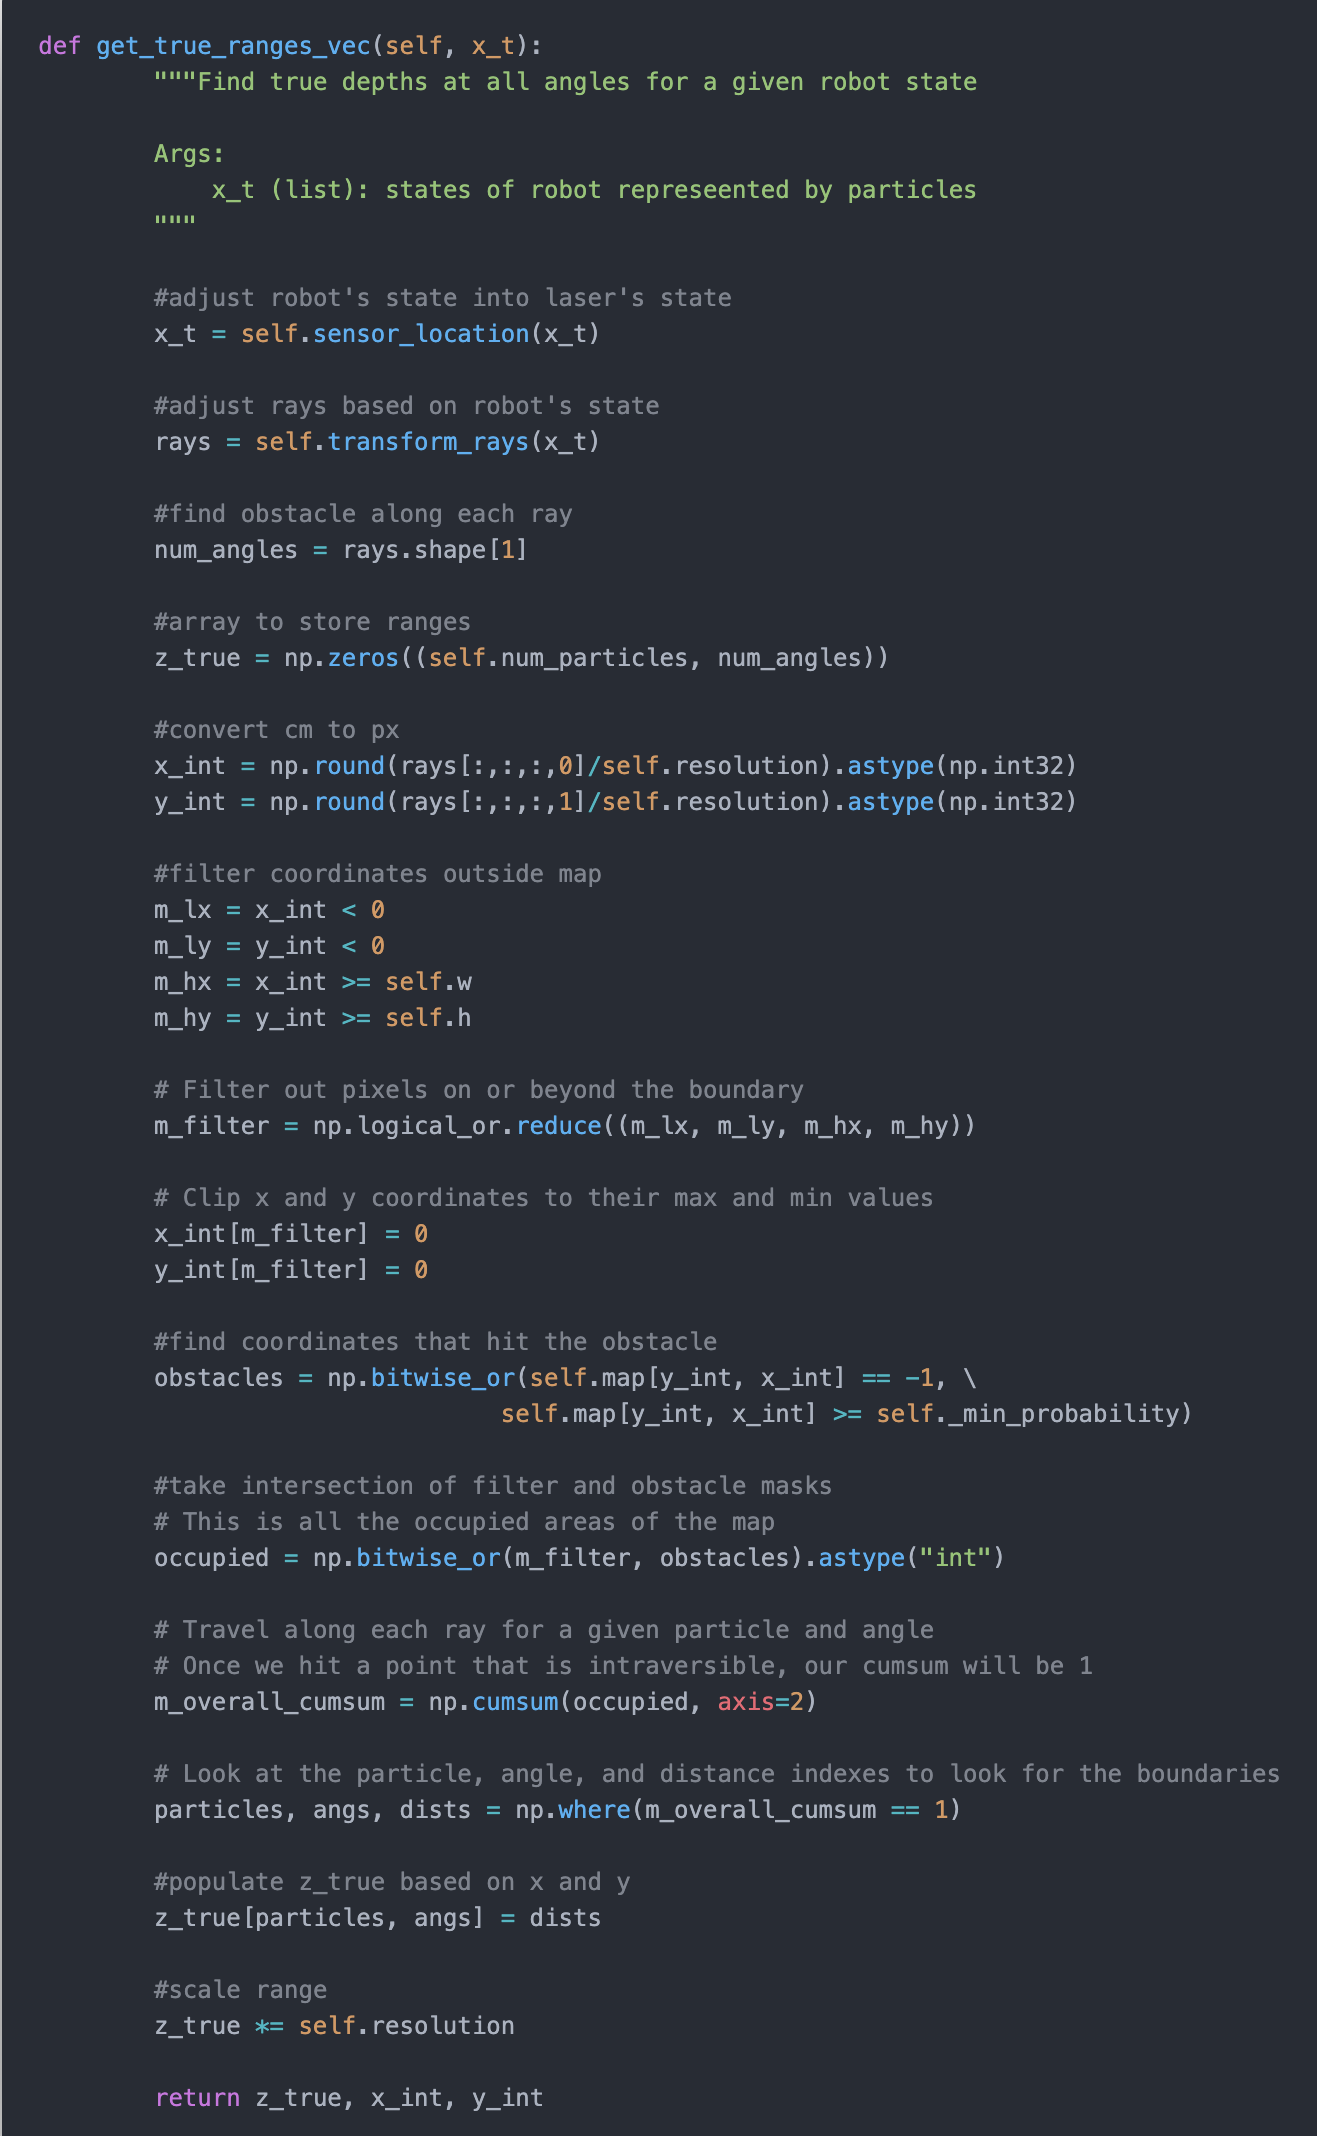
\includegraphics[scale=0.25]{./results/ray_casting_opt_2.png}
        \captionof{figure}{Vectorized logic to compute ranges}
        \label{fig:sm_1}
      \end{center}
    \end{minipage}
  \end{itemize}
\end{enumerate}

\subsection{Results}

The figure below shows rays cast from a sample robot state. The time taken to measure ground truth ranges at 36 angles for 1000 particles using our optimized implementation is just around \textbf{1.05 seconds} on Apple Macbook M1 Pro system.
\begin{figure}[H]
  \centering
  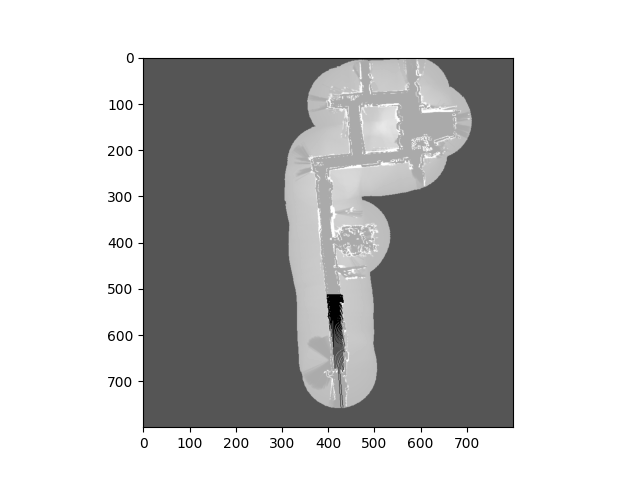
\includegraphics[width=0.9\linewidth]{results/ray_casting_2.png}
  \caption{Rays cast at a sample point and orientation}
\end{figure}
\subsection{Sensor Model}
\subsubsection{Description}
The Sensor Model is responsible for estimating how well each particle explains the observed range sensor data. For our implementation, we followed the range sensor model described in \cite{ProbRob} where the probability distribution of sensor measurement is modeled as a weighted average of four components that take into account randomness, presence of obstacles and errors in measurements leading to the sensor incorrectly measuring maximum range. These four components are shown in the figure below.\\\\
\begin{figure}[H]
  \centering
  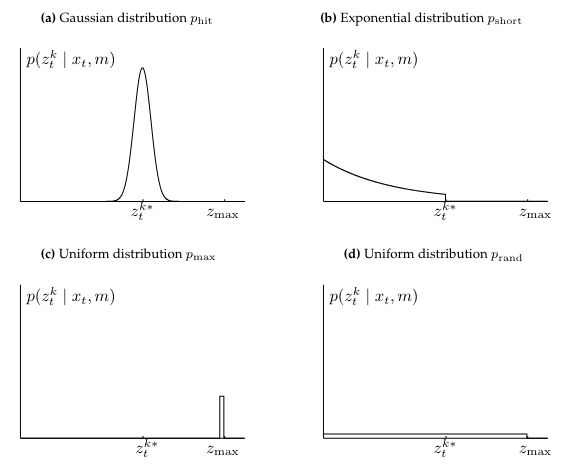
\includegraphics[width=0.9\linewidth]{results/sensor_model_pic.png}
  \caption{The four components of Sensor model}
\end{figure}

The Sensor Model has been implemented in \textit{SensorModel} class in \textit{sensor\_model.py}. The constructor accepts the occupancy map and number of particles as inputs.\\\\
The function \textit{beam\_range\_finder\_model} is called from \textit{main.py} everytime a laser reading is encountered. This function performs three important tasks:
\begin{enumerate}
  \item Get ground truth range readings using ray casting module
  \item Use ground truth and sensor readings to compute probabilities of each measurement for each particle
  \item Aggregate probabilities \textit{for} each particle using sum of logarithm of probabilities for numerical stability and then normalize probabilities \textit{across} particles using softmax operation to ensure that probabilities sum to 1.
\end{enumerate}
\subsubsection{Implementation}
\begin{figure}[H]
  \centering
  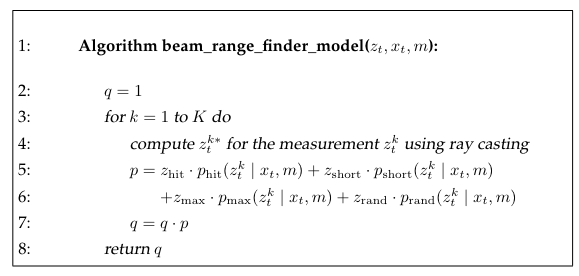
\includegraphics[width=0.9\linewidth]{results/sensor_model_desc.png}
  \caption{Description of Sensor model}
\end{figure}
The \textit{SensorModel} module takes up almost all ($99.1\%$ according to our estimates) of execution time. This makes optimization absolutely essential. We made the following changes to naive implementation to speed up the code:
\begin{enumerate}
  \item We vectorized the function \textit{beam\_range\_finder\_model} and all the functions it invokes to compute probabilities of all particles at once instead of invoking the function iteratively for each particle
  \item The functions to compute the four components of probability- \textit{p\_hit, p\_short, p\_max, p\_rand} have all been vectorized to compute probabilities for all particles simultaneously. An example is shown in figure below
  \begin{itemize}
    \item 
    \begin{minipage}[t]{\linewidth}
      \vspace{0pt}
      \begin{center}
        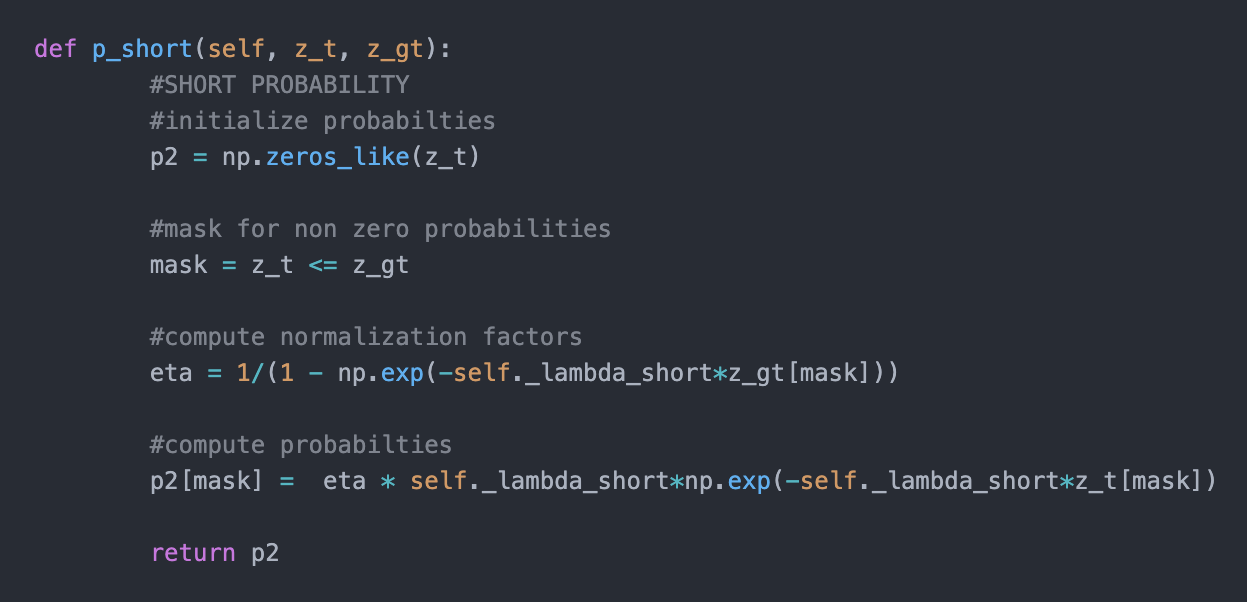
\includegraphics[scale=0.3]{./results/sensor_model_opt.png}
        \captionof{figure}{Vectorized probability computation}
        \label{fig:sm_1}
      \end{center}
    \end{minipage}
  \end{itemize}
\end{enumerate}



\section{Resampling}
The inherent nature of this algorithm is survivial of the fittest. Particles with a high probability realtive to the other particles, have a high chance of being retained. Meanwhile, low quality particles have a low probability of being maintained. However, if purely sampling by particle importance weights in a multinomial fashion, there is always an intrinsic variance or "luck" factor involved with random sampling. Therefore, we develop  low variance resampling algorithm mentioned in \cite{ProbRob} as follows:

\begin{figure}[H]
  \center
  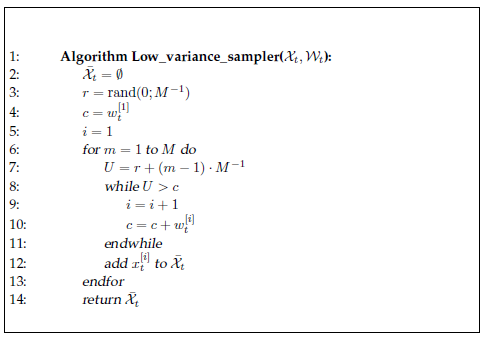
\includegraphics{LowVarianceResampling.png}
  \caption{Psuedo-Code for Low Variance Resampling \cite{ProbRob}}
\end{figure}

\noindent Notice in this implementation that only one random number is drawn and there is a constant step size before resampling each particle. This low variance variant ensures that highly probable particles have more of an guarantee of being sampled and can even be sampled multiple times if they are probable enough. This creates a necessity for parameter tuning but also allows for more consistency when resampling.

\begin{figure}[H]
  \centering
  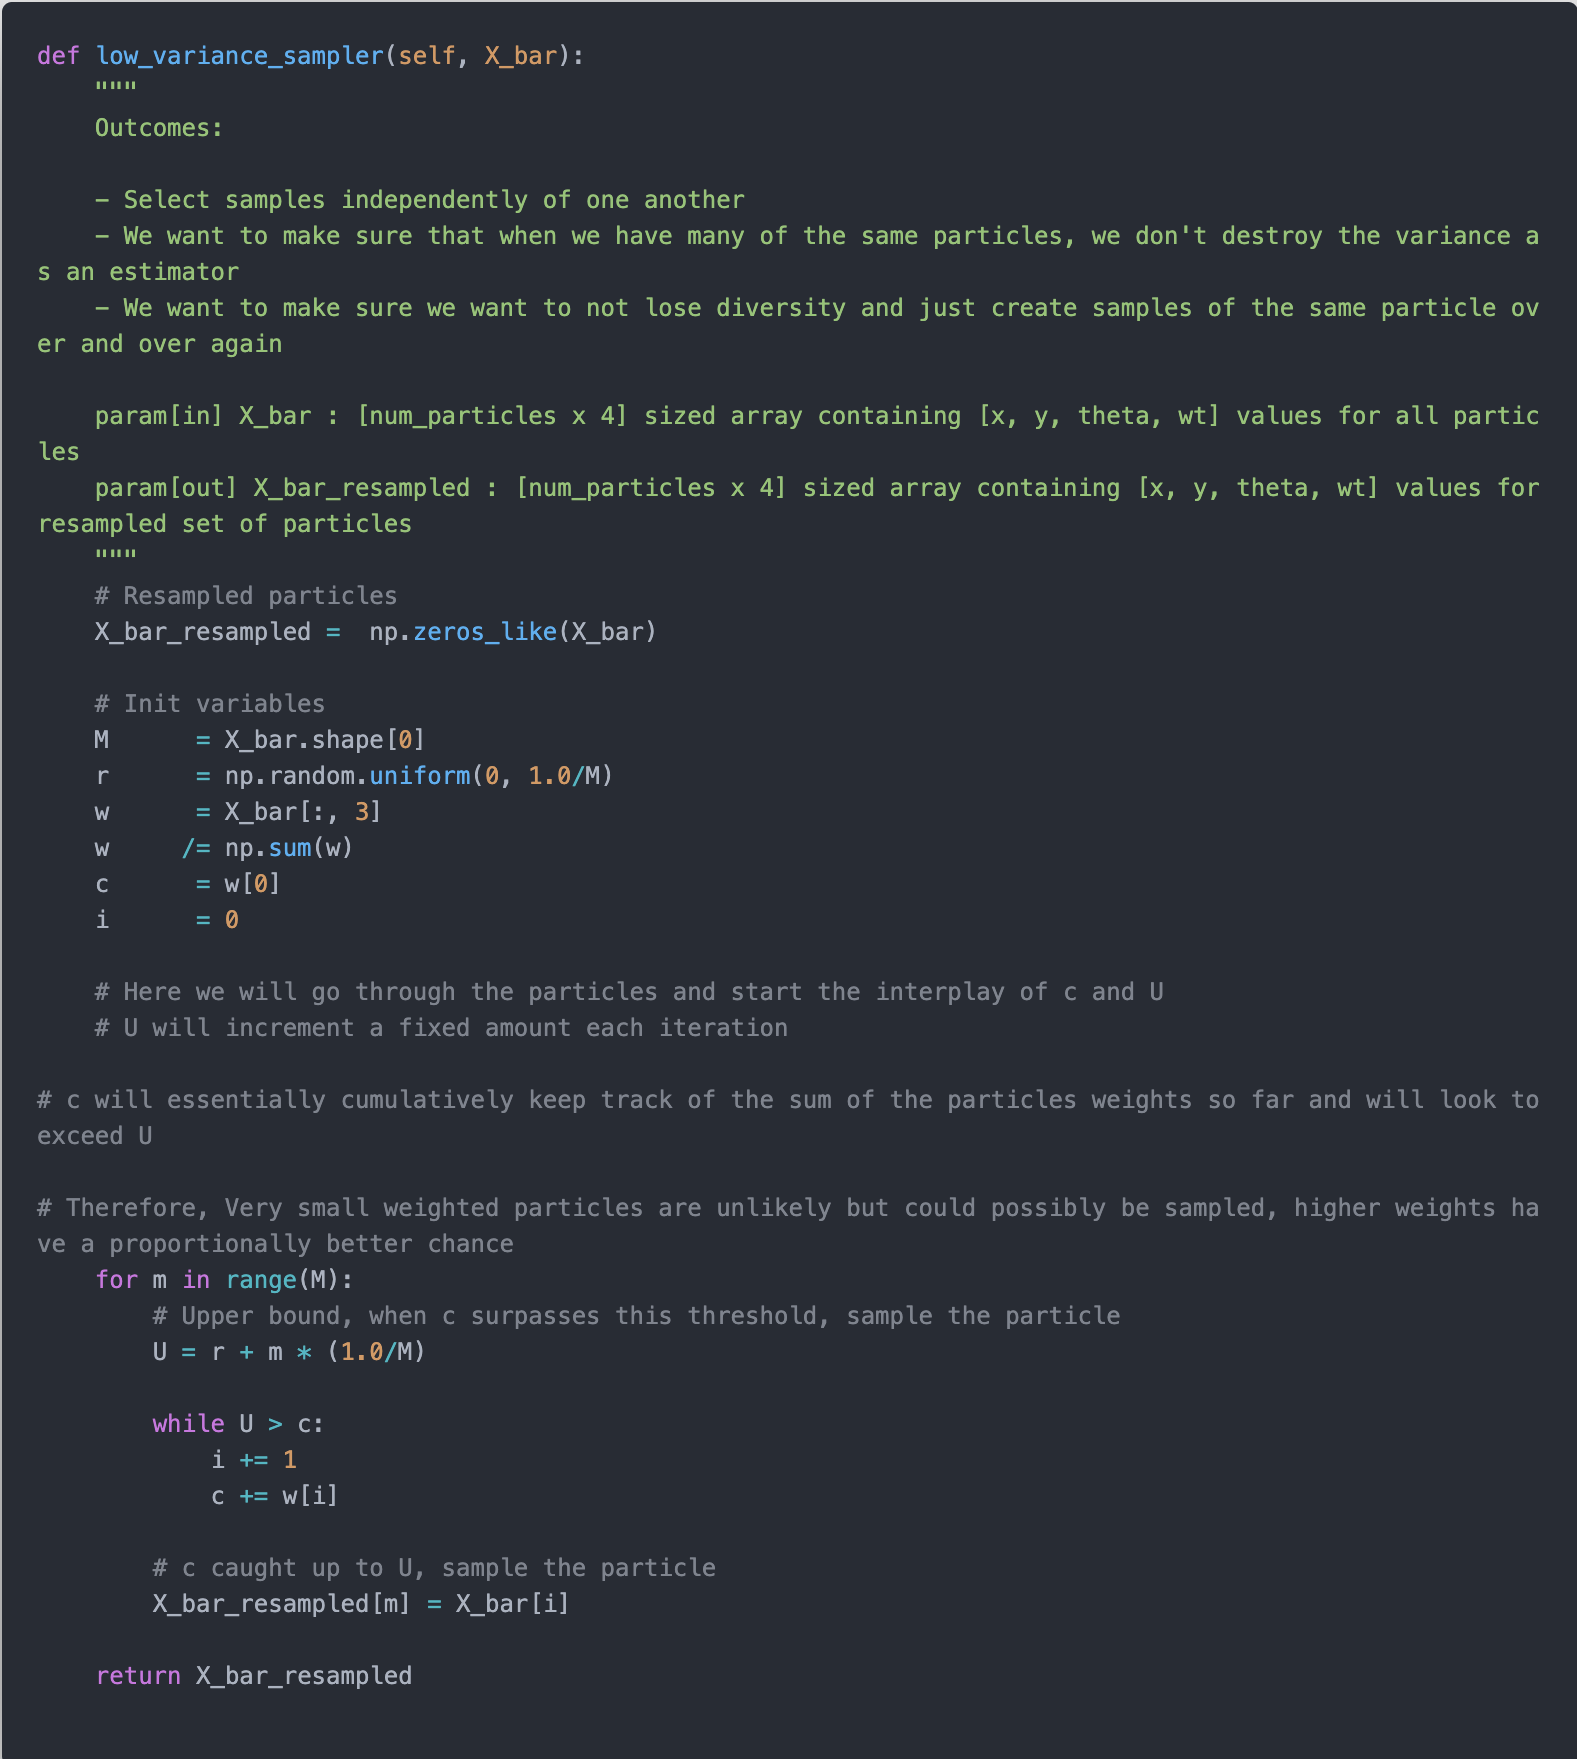
\includegraphics[width=0.9\linewidth]{results/resampling_2.png}
  \caption{Implementation of resampling}
\end{figure}
\subsection{Alterations}
Similar to the motion model, we do not perform resampling when the robot is not moving. We found this helps with algorithm speed and removes some noise during the "warmup" period

\[ 
x_{t} = \left\{
\begin{array}{ll}
    Low\_variance\_sampler(x_{t}, w_{t}) & \lVert u_{t1} - u_{t0} \rVert > \tau \\
    x_{t} & else
\end{array} 
\right. 
\]

\section{Performance}
The total time taken for execution of particle filter on \textit{robotdata1.log} with 1000 particles on Apple Macbook M1 Pro is \textbf{19.6 min}. The execution time without the optimizations in ray casting is more than 3 hours(180 min).
\begin{center}
  \begin{tabular}{|c|c|}
    \hline
    \textbf{Log File} & \textbf{Time(min)} \\
    \hline
    \textit{robotdata1.log} & 19.6 \\
    \hline
    \textit{robotdata2.log} &  63.5\\
    \hline
    \textit{robotdata3.log} &  34.7\\
    \hline
    \textit{robotdata4.log} &  17.1\\
    \hline
    \textit{robotdata5.log} &  27.5\\
    \hline
  \end{tabular}
\end{center}
\section{Parameter Tuning}
\subsection{Discussion}
Parameter tuning was undoubtedly the most rigorous and important part of the performance for this assignment. For the motion model, tuning $\alpha1$ and $\alpha_2$ had the most effect. A value that was too big caused jittering in the angle of the robot. A value that was too small caused the robot to not rotate enough. $\alpha_3$ and $alpha_4$ had a similar effect but for translation.\\

\noindent For the sensor model, the two most important parameters were $z_{rand}$ and $z_{hit}$. We used many different values for $z_{rand}$ but found the best performance when this was a large magnitude bigger than the other parameters. When $z_{rand}$ was too small, the particle clouds would collapse and certainly not converge. When $z_{rand}$ was too large, particles would stay alive for far too long and the measurements would have little impact. $z_{hit}$ had a similar effect, modelling our belief in the sensor providing the correct distance. When $z_{hit}$ was too small, there was little chance of convergence. When $z_{hit}$ was too large, there was too much belief in the measurements being made and would collapse potentially correct particle clouds.

\subsection{Final Parameters}
\subsubsection{Motion Model}
\begin{center}
\begin{tabular}{||c |c| c| c||} 
  \hline
  $\alpha_2$ & $\alpha_2$ & $\alpha_2$ & $\alpha_2$ \\
  \hline
  1e-4 & 1e-4 & 7.5e-4 & 7.5e-4 \\
  \hline
\end{tabular}
\end{center}

\subsubsection{Sensor Model}
\begin{center}
\begin{tabular}{||c | c | c | c | c | c||} 
  \hline
  $z_{hit}$ & $z_{short}$ & $z_{max}$ & $z_{rand}$ & $\sigma_{hit}$ & $\lambda_{short}$ \\
  \hline
  10 & 5 & 5 & 1000 & 75 & 0.5 \\
  \hline
\end{tabular}
\end{center}
\section{Results}
The results can be found at the links below. Our results match our observations based on the provided reference GIF \textit{robotmovie1.gif} for Log 1. However we suspect that there are errors in result on Log 2.\\\\
The errors could be due to our extremely optimized implementation of Ray Casting whose one drawback is introduction of quantization noise because we pre-compute all our rays and round particles along rays to integer coordinates on maps.\\\\
The Google Drive links to our videos are provided below. Please note that the video for Log 2 is at a 4x speed to reduce the run time from over 4 minutes to just over 1 minute.
\begin{center}
\begin{tabular}{||c | c||} 
  \hline
  Robot Log 1 & Robot Log 2 \\
  \hline
  \href{https://drive.google.com/file/d/1qt8UM7HHN9xPAYrRJYI5JoRR8iQb3wQ5/view?usp=sharing}{Log 1} & \href{https://drive.google.com/file/d/1-rfNtqJuf1p7kxYXcXjpizGDpsq9AJ4A/view?usp=sharing}{Log 2} \\
  \hline
\end{tabular}
\end{center}

\section{Future Work}
\begin{enumerate}
  \item As discussed in previous sections, our optimized ray casting performs 9.5x better than naive implementation. However there is scope for further improvement in performance with the use of GPUs that excel at matrix multiplications and additions
  \item Another interesting way to speed up ray casting algorithm that we haven't explored for the homework is to approximate all obstacles as a set of straight lines. Under this approximation, we just need to compute points of intersection of a set of lines and any given ray and choose one of the points of intersection as the obstacle. This requires a lot fewer computational resources than ray traversal. 
  \item Though we do well after tuning parameters, we still have occasional cases where we fail. For logs besides log 1, we are not as robust as we would like. We start to see the particles start to converge but then jump to the wrong location. I think we could get better results if we optimized for each log but that is not ideal in the slightest.
  \item In genreal, if we are in an area with more open space and less measureable landmarks, we may require different parameters. For this, having an adaptive number of particles and dynamic/learned parameter values may help. For the adaptive number of particles, as we increase and decrease confidence in the measurements around us, it would be ideal to add more particles to explore and reduce particles when we become more confident in our estimate. Furthermore, learned or adaptive parameters that could have a similar effect but may be able to infer about a shift in the sensor distribution and account for more hardware and noise related issues.
\end{enumerate}




\section{Extra Credit}
\subsection{Kidnapped robot problem}
The kidnapped robot problem presents a challenge to robot localization problem since the particles in particle filter tend to concentrate around robot's location. This means that when a robot is kidnapped and taken to a new location, is is highly likely that there are no particles around the robot's new location.\\\\
This will cause the particle filter to continue to believe that it is in it's pre-kidapping location and not adjust to it's new position. We can think of two ways to deal with this problem
\begin{enumerate}
  \item Randomly distribute a small fraction of the particles all over the map inspite of the outcome of particle filter. This will increase the chance of presence of a particle near robot's new location and thereby increase the likelihood that the robot will adjust to it's new surroundings
  \item When a robot is taken to a new location, the sensor readings taken immediately after being placed in the new location will not align with the particles which are still concentrated around the previous state of robot before it was kidnapped. Therefore, one way to detect the kidnapping of a robot is by computing a metric that measures the compatibility of current sensor readings with previous particle states. One such measure could simply be the likelihood $p(z_t|x_t)$ estimated by the sensor model. When the robot is transported to a new location, it is reasonable to assume that $p(z_t|x_t)$ will drop suddenly. Therefore, kidnapping of a robot can be identified when there is a sudden drop in likelihood estimates measured by sensor model. Once the kidnapping has been identified, we can re-initialize particles to random locations to help the robot identify it's new location.
\end{enumerate}

\subsection{Adaptive Number of Particles}

While implementing this homework, we found increasingly that a high number of particles are extremely useful in the "warmup period" of obtaining sensor readings, it is not as useful once the algorithm is close to convergence. Many of the particles are redundant and will not be useful unless more divergent paths appear (the particles are closer to a uniform distribution).\\

\noindent From these observations, we present the idea of analyzing the entropy of the particles' probabilities in order to inform our algorithm if we need more or less particles. The entropy acts as a level of uncertainity about the distriubtion, with 0 being a single particle with all the probability and 1 being a uniformly distributed particle set. We define entropy w.r.t. weights $w_t^{(i)}$ as:

$$ H(w_t) = - \sum_{i=1}^{M} log(w_t^{(i)})w_t^{(i)} $$


\noindent However, entropy by itself is not suitable. It may be more convenient to utilize the entropy at two consecutive timesteps and calculate the the information gain from frame t to frame t+1:
If our entropy is low, we want to reduce the number of particles


\noindent In the first frame, we have particles that are all evenly weighted. As our probability distribution shifts, we want to adjust the number of particles by whether the difference in entropy (or information gain) is positive or negative. If positive, that means we have become more uncertain so we need to increase the number of particles. If negative, that means we are become less certain so we need to decrease the number of particles.
We define the formula to calculate number of particles as:

$$M = Me^{H(w_{t_1}) - H(w_{t_0})}$$

\noindent If there is no information gained, the number of particles will stay the same. If the entropy increases, more particles will be added, if the entropy decreases, particles will be removed.\\

\noindent A few implementation details include the frequency of changing the number of particles. Our initial experimentation had a max frequency of 2. That is, at most, the number of particles would change every other time step. This was done to ensure that we are not artifically inflating the entropy by adding more particles. Therefore, we only calculate information gain when two timesteps have the same number of particles. Lastly, we enforce a minimum number of particles of 50 to ensure our particles do not drop too low.

\begin{figure}[H]
  \centering
  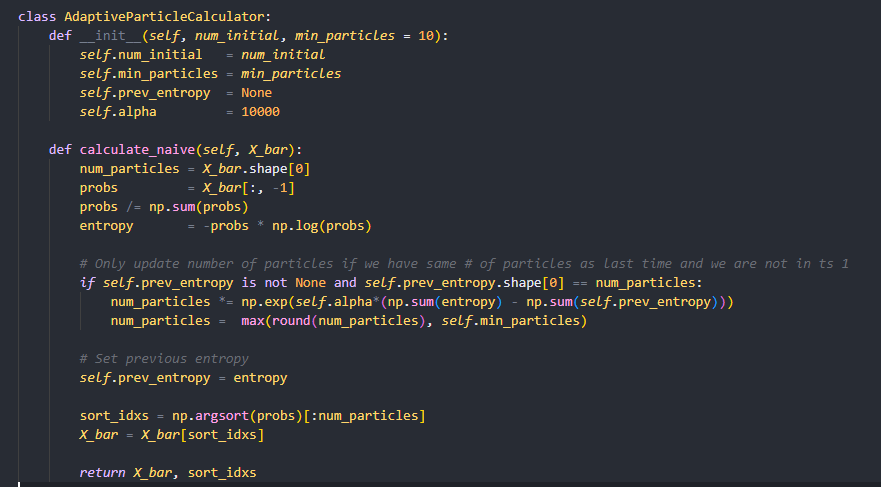
\includegraphics[width=0.9\linewidth]{results/adaptive_particles.PNG}
  \caption{Code for adaptive particles}
\end{figure}

\begin{thebibliography}{9}
  \bibitem{ProbRob}
  Sebastian Thrun, Wolfram Burgard, and Dieter Fox (2005) \emph{Probabilistic Robotics}, MIT Press
\end{thebibliography}

\end{document}

\end{document}